\documentclass[conference]{IEEEtran}
\IEEEoverridecommandlockouts
\usepackage{cite}
\usepackage{amsmath,amssymb,amsfonts}
\usepackage{graphicx}
\usepackage{textcomp}
\usepackage{booktabs}
\usepackage{multirow}
\usepackage{tipa}
\usepackage{xcolor}
\usepackage{tikz}
\usetikzlibrary{positioning,arrows.meta,shapes.geometric,fit,calc}
\usepackage[T1]{fontenc}
\newcommand{\tbd}[1]{\textcolor{red}{[TBD: #1]}}
\newcommand{\ipa}[1]{/#1/}

\begin{document}

\title{Visual Pronunciation Feedback for Deaf and Hard-of-Hearing Learners of English Consonants: A Feasibility Study of Recogniser-Assisted Scoring\\
\tbd{working title}}

\author{\IEEEauthorblockN{Kiet Pham}
\IEEEauthorblockA{\textit{\tbd{department}} \\
\textit{National Formosa University}\\
tuankiet.work.2909@gmail.com}
\and
\IEEEauthorblockN{Quang Nguyen}
\IEEEauthorblockA{\textit{\tbd{department}} \\
\textit{National Formosa University}\\
nmq.brian@gmail.com}
\and
\IEEEauthorblockN{Hui-Kai Su}
\IEEEauthorblockA{\textit{\tbd{department}} \\
\textit{National Formosa University}\\
\tbd{email}}
}

\maketitle

\begin{abstract}
\normalfont\mdseries
Deaf and Hard-of-Hearing learners may have limited opportunities to receive auditory feedback as they work on their English pronunciation, especially consonant sounds. This paper describes a web-based prototype dealing with eight English consonants, which includes two different applications: one aimed at providing DHH learners with visual feedback and guided practice, and another web-based platform designed for researchers and teachers to examine recordings, acoustic measurements, and assessment outcomes. The application used by learners combines diagrams showing the correct articulation, mouth cues obtained from a camera, and real-time acoustic guidance for certain consonants, together with judgements after the recording has been made regarding whether the pronunciation was ``correct'', ``almost'', or ``not yet''. The analytical application offers spectrograms and other interpretable acoustic data such as the spectral centre of gravity (CoG), voice onset time (VOT), and relative frication level. A multilingual phone recogniser is used to identify the consonants, and the acoustic measurements are then used to give graded feedback. The technical evaluation makes use of native speech from the CMU ARCTIC database and human-annotated second-language speech from the L2-ARCTIC database. On the L2-ARCTIC data, the use of the recogniser in scoring reduced the false rejection rate of correctly produced /s/ and /\textesh/ from 45\% and 43\% to 8\% and 3\%, respectively, while it detected 100\% and 88\% of the annotated substitutions. These results indicate that it is technically feasible to combine accessible feedback for learners with detailed analysis for researchers and teachers. The prototype is meant to help DHH children carry out independent pronunciation practice after they have received initial guidance and as part of teacher-led pronunciation intervention.
\end{abstract}

\begin{IEEEkeywords}
assistive technology, deaf and hard-of-hearing, pronunciation feedback, universal design for learning, phone recognition
\end{IEEEkeywords}

\section{Introduction}
Pronunciation of a second language depends strongly on auditory feedback, and it is therefore a particular barrier for DHH learners. English fricatives such as /s/, /\textipa{S}/, and /f/ differ in their spectral characteristics and amplitude \cite{jongman2000}. Access to high-frequency information is particularly relevant to the perception of /s/, for which recognition varies with stimulus bandwidth, hearing status, and talker characteristics \cite{stelmachowicz2001}. Consequently, a learner may produce ``see'' as ``she'' without noticing the difference, whereas a teacher cannot attend to every learner continuously. If the visual modality can replace the auditory one, learners are able to practise independently.

Automatic pronunciation feedback has been studied extensively, yet it is usually developed and validated on native speech that is pronounced correctly. However, the intended users of an assistive tool are learners whose productions differ systematically from native speech, and the cost of an incorrect judgement is high: a correct production marked as wrong discourages a learner who has no independent means of verifying the result. It is therefore necessary to determine whether feedback that is valid for native speakers remains valid for learners.

The present study addresses this question for eight English consonants (\ipa{s}, \ipa{\textesh}, \ipa{f}, \ipa{t\textesh}, \ipa{m}, \ipa{n}, \ipa{p}, \ipa{b}). The contributions are as follows.
\begin{enumerate}
\item A web-based visual feedback tool is described, designed according to the principles of Universal Design for Learning (UDL) so that every judgement is presented through several representations (colour mark, spectrogram, numerical measures, and a written tip).
\item It is shown, on human-annotated learner errors, that fixed acoustic thresholds validated on native voices over-reject correct learner speech, and a recogniser-assisted design that reduces this error is proposed and evaluated.
\item An evaluation protocol is described, comprising leave-one-speaker-out testing, annotated L2 errors, and context-controlled recogniser tests, together with the limitations that remain before classroom use.
\end{enumerate}

\section{Related Work}
\textit{Visual feedback for speech training.} Visual--acoustic biofeedback, in which the learner matches a live acoustic representation, such as a linear predictive coding spectrum, to a target, is an established clinical technique for residual speech sound errors, and a recent tutorial states that its success depends on the comprehension of the representation by clinician and client, on the choice of the acoustic target and template, and on the practice schedule~\cite{hitchcock2023}. These requirements motivate a display in which the learner is not required to interpret a spectrum, and in which a categorical mark accompanies the signal.Visual feedback can offer DHH learners an additional method for observing and comparing their productions with target patterns by making aspects of speech production visible \cite{hitchcock2023}. This feedback may also encourage independent practice of pronunciation \cite{ertmermaki2000} following initial instruction. 

\textit{Consonant perception and production in DHH learners.} For listeners with hearing impairment, visual cues contribute more to the identification of consonants than of vowels~\cite{moradi2017}, and cochlear-implant (CI) users rely more strongly on the visual cue than normal-hearing listeners when the auditory cue is weak~\cite{desai2008}. CI listeners can also use visual information to accommodate the acoustic differences between \ipa{s} and \ipa{\textesh} across talkers~\cite{winn2013}, and deaf adults with CIs retain a speechreading skill that is not inferior to that of hearing adults~\cite{pimperton2017}. With respect to production, young CI recipients produce initial consonants with lower accuracy and greater variability than typically developing peers, and fricatives and affricates are acquired later than stops and nasals~\cite{ertmer2011}. Collectively, the findings above highlight a need for the development of visual feedback to facilitate English consonant practiced  by DHH students, where the feedback is meant to be simplified.

\textit{Visual Feedback and Guidance for DHH Learners} 

\textit{Automatic detection of L2 pronunciation errors.} Acoustic--phonetic classifiers trained for specific frequently mispronounced sounds, with linear discriminant analysis and decision trees, were able to discriminate correct from incorrect productions in native and non-native speech, whereas confidence measures from speech recognisers are less accurate predictors of phone-level quality~\cite{truong2005}. The present design combines both families: a recogniser decides which sound was produced, and interpretable acoustic measures determine its degree. Self-supervised representations have furthermore been shown to predict the intelligibility of L2 talkers over and above traditional acoustic--phonetic cues~\cite{kim2025}, which supports the use of recogniser features, such as the linear probes of the present study, for learner speech. The recogniser is a wav2vec~2.0 model~\cite{baevski2020} fine-tuned for multilingual phone recognition~\cite{xu2022}, and the acoustic characterisation of English fricatives follows the spectral-moment approach~\cite{jongman2000}. Learner errors are taken from L2-ARCTIC~\cite{zhao2018}.

\textit{Word selection.} The target words (\textit{see}, \textit{she}, \textit{fee}, \textit{pea}, \textit{bee}, \textit{me}, \textit{knee}, \textit{cheat}) are common monosyllabic words; large-scale age-of-acquisition ratings~\cite{kuperman2012} can be used to verify that they are acquired early. \tbd{Check the ratings of the eight words and report them, or drop this sentence.}

\textit{}

\tbd{Broaden with computer-assisted pronunciation training (CAPT) and mispronunciation-detection literature (e.g., goodness-of-pronunciation scoring), commercial pronunciation tools, and UDL in language learning; the present section cites only the sources supplied so far.}

\section{System and Method}
\subsection{Interaction Design}
The learner selects a target word (for example, \textit{see}, \textit{she}, \textit{fee}, \textit{pea}, \textit{me}, \textit{cheat}) and records it or uploads a file. The tool returns a Japanese-style grading mark (\textit{correct}, \textit{almost}, \textit{not yet}) with a written tip and an articulation diagram of the target sound. Below the verdict, the spectrogram with the detected consonant, the numerical measures, and a comparison with reference voices are displayed, so that a teacher or learner can inspect the basis of the judgement. A calibration page, in which the learner records \textit{see}, \textit{she}, and \textit{fee} twice each, adapts the scoring to the individual voice. Fig.~\ref{fig:pipeline} gives an overview.


\begin{figure*}[!t]
\centering
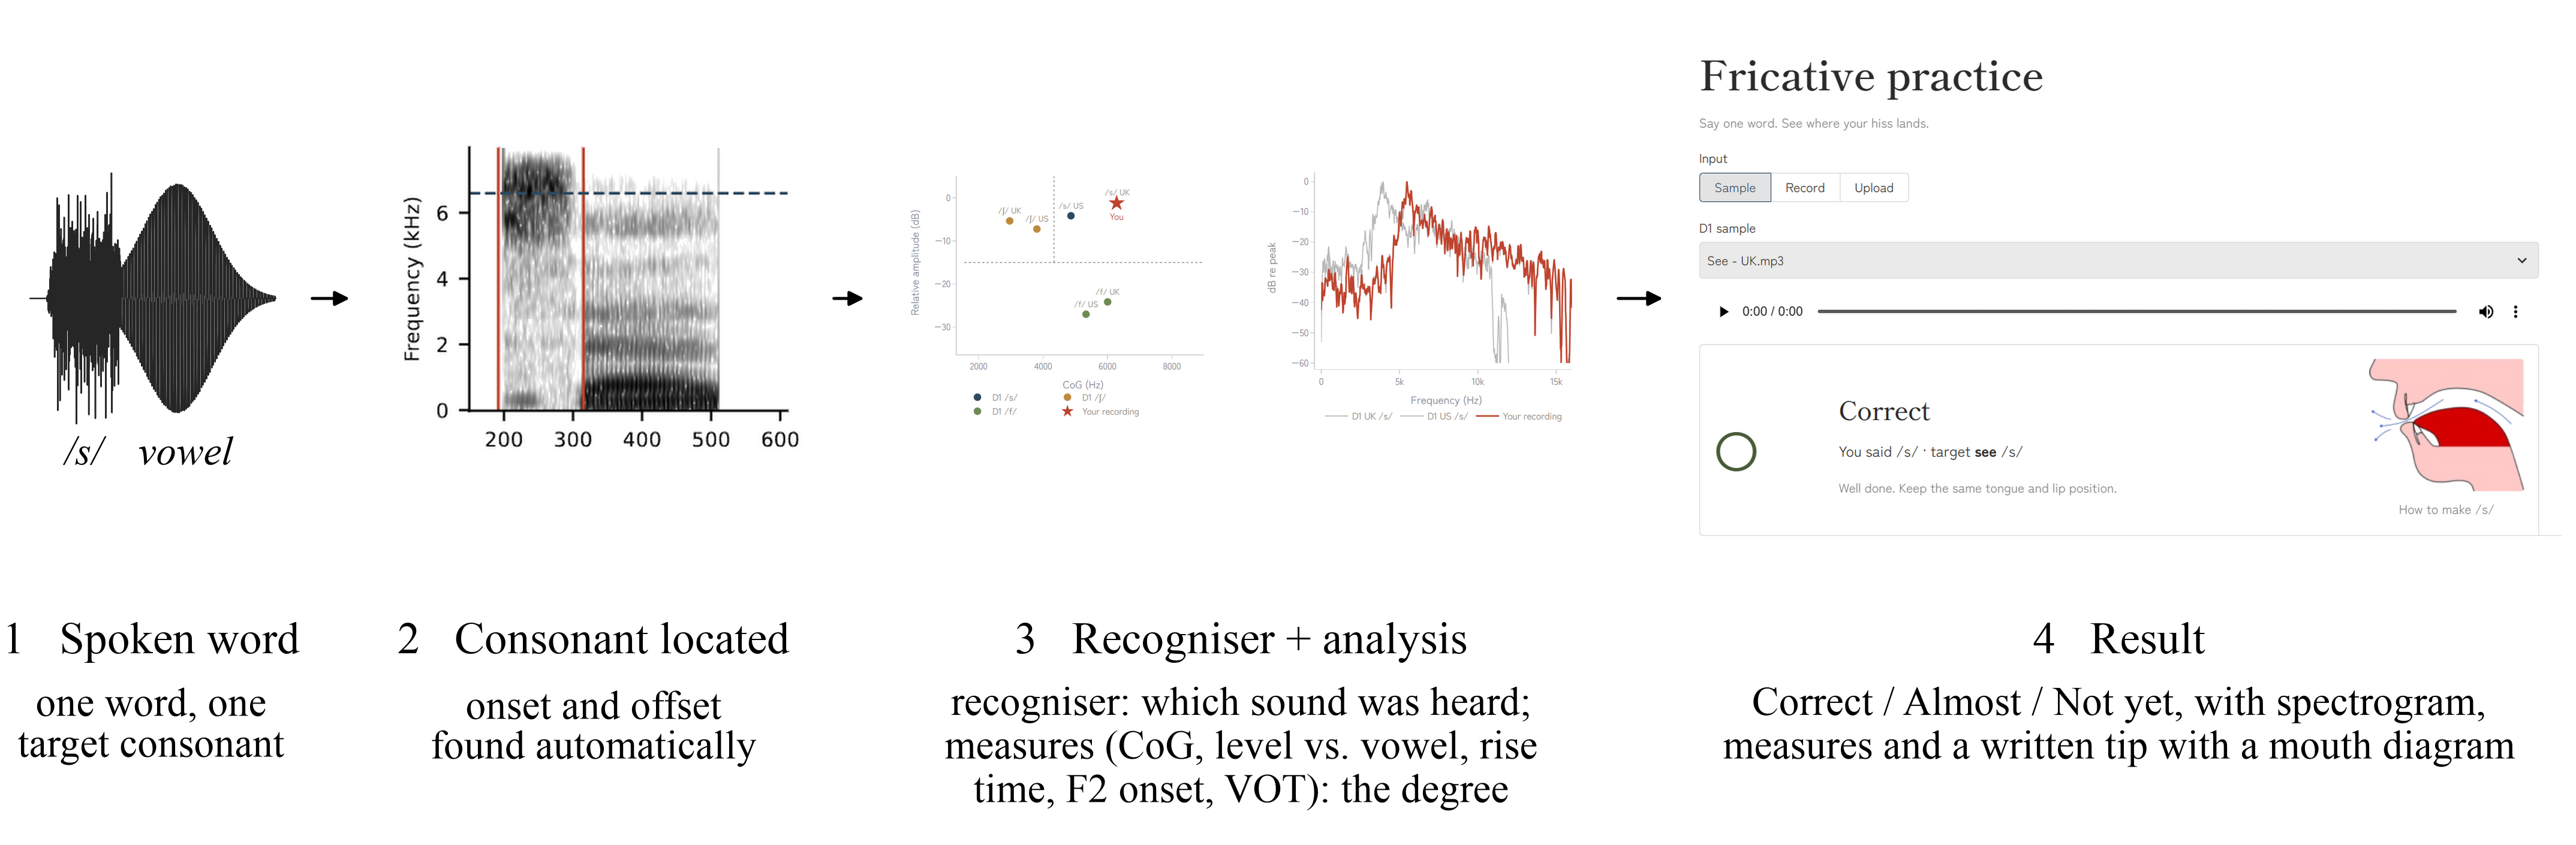
\includegraphics[width=\textwidth]{figs/Figur1.png}
\caption{Overview of the feedback tool. (1)~The learner selects a target word and records or uploads it. (2)~The web tool locates the target consonant. (3)~A multilingual phone recogniser decides whether the intended sound was produced, and acoustic measures determine the degree of correctness. (4)~The learner receives a three-level judgement together with a spectrogram, numerical measures, and a written tip; every judgement is presented through several representations, following Universal Design for Learning (UDL). Panel~4 shows a sample application result.}
\label{fig:pipeline}
\end{figure*}

\subsection{Consonant Location and Acoustic Measures}
For fricatives, the onset is the start of the run of high-band energy (2.5--12~kHz) that precedes the vowel, with a frame counted as part of the run when it lies at least 15~dB above the noise floor of the recording itself, and the offset is the first voiced frame. The centre of gravity (CoG) is computed on the middle 50\% of this segment with a rectangular window and a spectral power of two, which is the setting of the manual Praat measurements used as reference. The hiss level relative to the following vowel separates \ipa{f} from the sibilants. For \ipa{p} and \ipa{b}, the voice onset time (VOT) is the interval between the burst, detected in the 1.5--7.5~kHz band, and the first voiced frame. For \ipa{t\textesh}, the rise time and steepness of the hiss envelope are used.

\subsection{Recogniser-Assisted Scoring}
A multilingual phone recogniser (wav2vec~2.0 XLSR-53 fine-tuned on eSpeak phone transcriptions~\cite{baevski2020,xu2022}) is applied to the segment located above. The posterior probabilities of the phones belonging to each sound class are averaged over the consonant, and the class with the highest mean posterior is taken as the sound heard. The design principle is a division of labour: the recogniser decides whether the intended sound was produced, whereas the acoustic measures decide between \textit{correct} and \textit{almost}. When the recogniser hears a different sound, the verdict is \textit{not yet}; when it hears the intended sound but the thresholds disagree, the verdict is \textit{almost}. A gate based on the first decoded phone additionally withholds scoring when a different kind of sound (for example, a fricative for a stop target) is heard. For \ipa{p}--\ipa{b}, a logistic probe on the mean layer-8 hidden state over the release is used, and for \ipa{t\textesh}--\ipa{\textesh} a corresponding probe over the hiss.

\subsection{Calibration to the Learner}
Every feature is expressed as a z-score relative to six calibration recordings of the learner, and a shrinkage linear discriminant model, trained on eight native voices normalised in the same way, estimates the probabilities of \ipa{s}, \ipa{\textesh}, and a weak hiss. This component is optional and is not used by the recogniser branch.

\section{Data Collection and Processing}
\subsection{Corpora}
Table~\ref{tab:corpora} summarises the four sources. Dictionary recordings (D1) provide manual reference values. The native-speaker experiments use the CMU ARCTIC corpus~\cite{kominek2004}, whose phone labels were produced by forced alignment and have not been verified manually. The L2-ARCTIC corpus~\cite{zhao2018} provides the only human-annotated learner errors. Recordings of isolated words by native, L2, and DHH speakers (D2 and D3) are planned and have not yet been collected; DHH recordings are conditional on ethical approval and informed consent. \tbd{Describe the D2/D3 recording script, number of speakers, equipment, and consent procedure once fixed.}

\begin{table}[!htb]
\caption{Data sources.}
\label{tab:corpora}
\centering
\footnotesize
\begin{tabular}{p{1.6cm}p{2.9cm}p{3.1cm}}
\toprule
Source & Content & Role \\
\midrule
D1 & 6 dictionary words (\textit{see}, \textit{she}, \textit{fee}; UK, US) with manual Praat boundaries and CoG & Agreement with manual measurement \\
ARCTIC~\cite{kominek2004} & 8 native US voices (4 male, 4 female), 300--590 sentences each, forced-aligned phones & Training and leave-one-voice-out tests \\
L2-ARCTIC & 24 speakers, 6 first languages (4 Vietnamese); 3{,}599 utterances with human annotation of substitutions & Detection of annotated learner errors \\
D2, D3 & Isolated words by native, L2, and DHH speakers \tbd{planned} & Final validation \\
\bottomrule
\end{tabular}
\end{table}

\subsection{Token Extraction and Pre-processing}
Corpus audio was resampled to 16~kHz, which is the analysis rate of ARCTIC and bounds the usable spectrum at 8~kHz. A token was defined as a word-initial consonant of one of the eight classes followed by a vowel of at least 50~ms, and its duration was required to be at least 20--40~ms depending on the class. The token, together with the following vowel, was cut from the sentence and embedded between 0.2~s of silence and 0.1~s of silence with low-level noise, in order to approximate an isolated word recorded after a short pause. The resulting numbers are given in Table~\ref{tab:summary}. In the application itself, recordings are decoded with Parselmouth (a Python interface to Praat), converted to mono, and limited to the first five seconds.

\subsection{Evaluation Procedure}
Native-speaker accuracy was estimated by leave-one-voice-out testing with balanced accuracy. Learner speech was scored with the same code as the application, and the result was compared with the annotation (substitution or correct). Two rates are reported: the false-rejection rate (FR), defined as the share of correctly produced consonants marked \textit{not yet}, and the detection rate (Det.), defined as the share of annotated substitutions marked \textit{not yet}. Wilson 95\% intervals are given, because the number of annotated errors is small for several sounds; Fig.~\ref{fig:eval} summarises the workflow. \tbd{Fig.~\ref{fig:eval} lists a confusion matrix among the metrics, but none is reported; add one or edit the figure. It also says leave-one-speaker-out for learner speech, whereas learner speakers are only split into a development and a test group so far; the unified evaluation (running) is to replace the current learner numbers. The word ``effectiveness'' in step~4 should read ``feasibility'', since no learning outcome is measured.} Three controls address the unit of evaluation for the recogniser: the consonant alone, the consonant with surrounding context, and the hiss of one sound spliced into a word of another.

\begin{figure*}[!t]
\centering
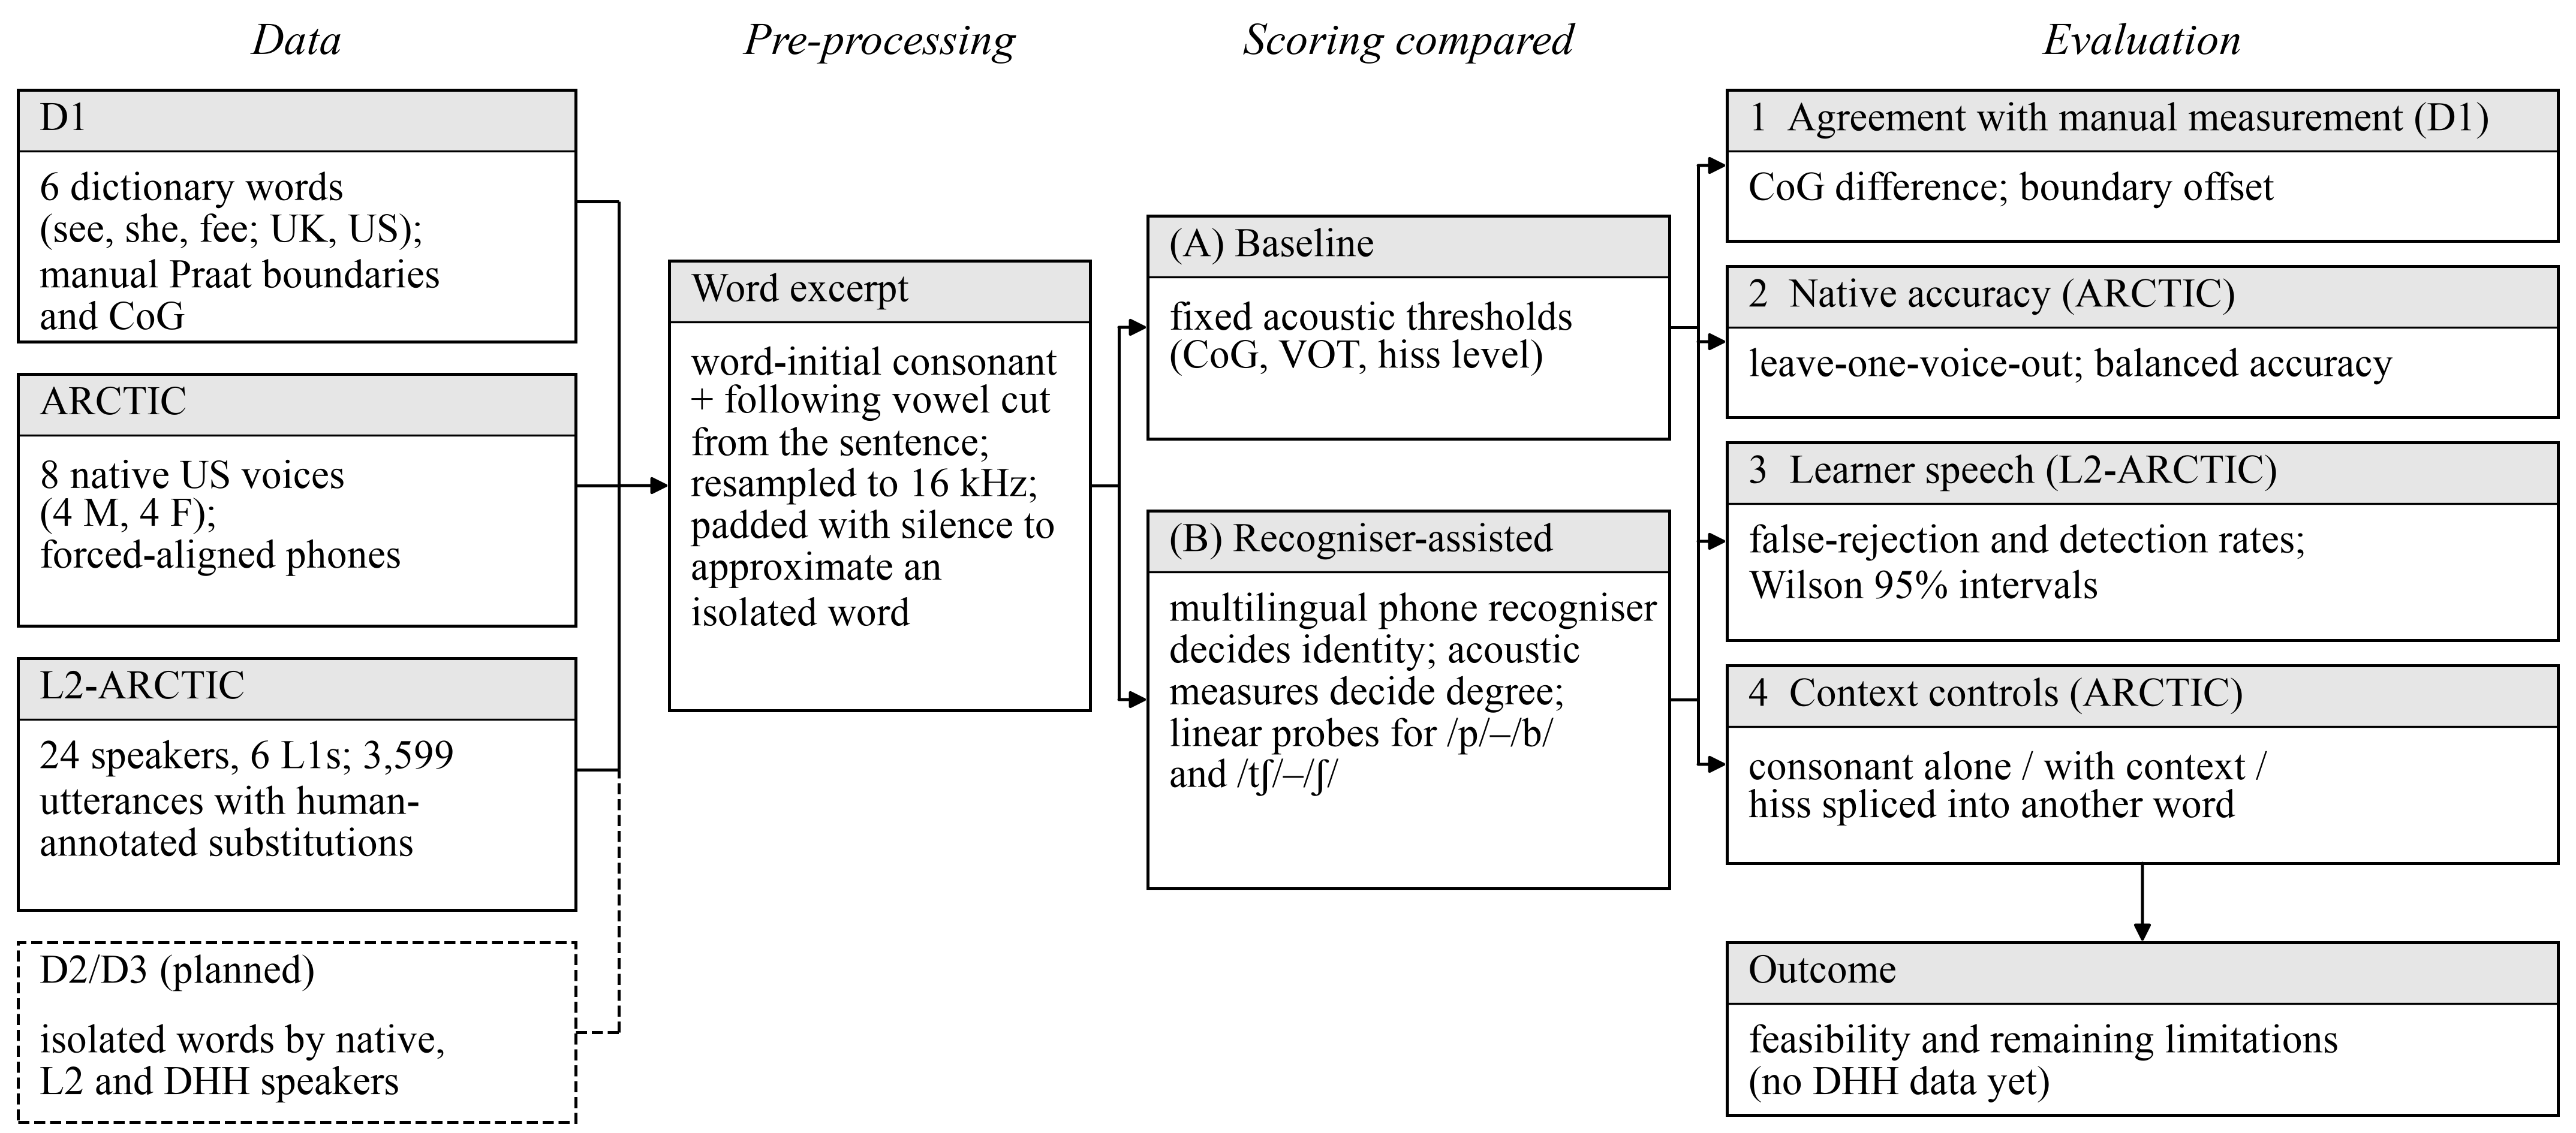
\includegraphics[width=0.72\textwidth]{figs/Figure 2.png}
\caption{Evaluation workflow. Native reference speech and annotated learner speech are collected, the test protocol combines leave-one-speaker-out testing, annotated L2 errors, and context-controlled recogniser tests, the baseline of fixed acoustic thresholds is compared with the recogniser-assisted design using accuracy and false-rejection rate, and the analysis identifies the remaining limitations.}
\label{fig:eval}
\end{figure*}

\section{Results}
\subsection{Summary for All Eight Sounds}
Table~\ref{tab:summary} lists, for each sound, the target words, the scoring method of the current prototype, the accuracy on native speech, and the behaviour on annotated learner speech. Two points should be noted. First, native accuracy is high for all sounds except \ipa{f}, for which only a weak hiss can be distinguished from the sibilants and the contrast with \ipa{\texttheta} is not established. Second, learner error counts are very small for \ipa{f}, \ipa{m}, \ipa{n}, and \ipa{t\textesh}, so that their detection rates are not interpretable.

\begin{table*}[!t]
\caption{Summary by sound. Native accuracy: balanced accuracy, leave-one-voice-out, ARCTIC. L2: L2-ARCTIC; FR = false rejection of correct productions, Det. = detection of annotated errors, percentages with Wilson 95\% intervals; $n$ = correct / error.}
\label{tab:summary}
\centering
\footnotesize
\begin{tabular}{lllcccc}
\toprule
Sound & Target words & Scoring method & Native acc. & L2 $n$ & L2 FR (\%) & L2 Det. (\%) \\
\midrule
\ipa{s} & see, sip, sun & Recogniser identity + CoG/LDA degree & 0.95\textsuperscript{a} & 861 / 18 & 8 [6, 10] & 100 [82, 100] \\
\ipa{\textesh} & she, ship, shoe & Recogniser identity + CoG/LDA degree & 0.95\textsuperscript{a} & 602 / 32 & 3 [2, 5] & 88 [72, 95] \\
\ipa{f} & fee, fan, food & Recogniser identity + relative level & 0.93\textsuperscript{b} & 1160 / 1 & 11 [9, 13] & n/a (1 error) \\
\ipa{t\textesh} & cheat & Probe on hiss vs.\ \ipa{\textesh} & 0.96\textsuperscript{c} & 267 / 5 & 7 [5, 11] & 20 [4, 62] \\
\ipa{m} & me & Recogniser at the nasal & 0.98\textsuperscript{d} & 1205 / 0 & 1 [1, 2] & n/a (0 errors) \\
\ipa{n} & knee & Recogniser at the nasal & 0.98\textsuperscript{d} & 682 / 3 & 1 [0, 2] & 33 [6, 79] \\
\ipa{p} & pea & Probe on release (VOT fallback) & 0.96\textsuperscript{e} & 309 / 86 & 36 [31, 41] & 85 [76, 91] \\
\ipa{b} & bee & Probe on release (VOT fallback) & 0.96\textsuperscript{e} & 962 / 26 & 10 [8, 12] & 54 [35, 71] \\
\bottomrule
\multicolumn{7}{l}{\scriptsize \textsuperscript{a}\ipa{s}--\ipa{\textesh}, calibrated, end-to-end (CoG alone: 0.87 uncalibrated, 0.93 normalised). \textsuperscript{b}weak hiss against sibilants, end-to-end; \ipa{f}--\ipa{\texttheta} not distinguished (0.67 on the hiss alone).} \\
\multicolumn{7}{l}{\scriptsize \textsuperscript{c}\ipa{t\textesh}--\ipa{\textesh}, end-to-end (hand-crafted features: 0.80). \textsuperscript{d}\ipa{m}--\ipa{n} (Praat formants: 0.63). \textsuperscript{e}\ipa{p}--\ipa{b} (VOT rule: 0.88 end-to-end).} \\
\end{tabular}
\end{table*}

\subsection{Agreement with Manual Measurement}
On D1, the CoG computed by the tool differed from the manual Praat values by less than 2~Hz, the automatic boundaries lay within 20~ms of the manual boundaries, and all six recordings were assigned to the correct sound. This agreement, however, concerns two dictionary voices only.

\begin{figure*}[!t]
\centering
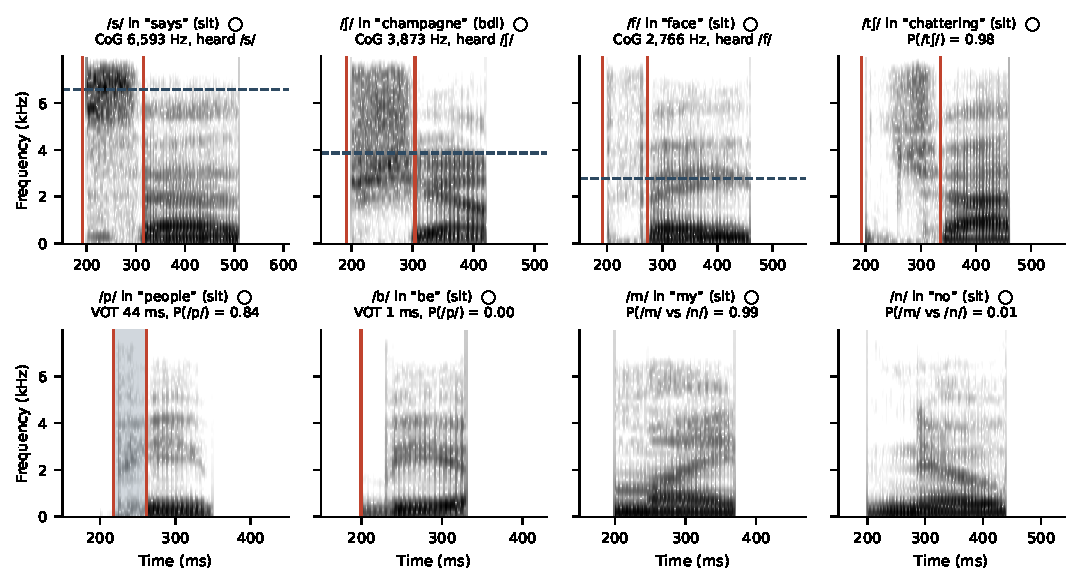
\includegraphics[width=\textwidth]{figs/fig_all_sounds.pdf}
\caption{Full spectrograms (0--8~kHz) of one correctly produced token of each of the eight sounds (native ARCTIC voices, sentences not used for training), cut like an isolated word, with what the tool detected: red lines mark the detected hiss (fricatives, \ipa{t\textesh}) or the burst and the start of voicing (stops), the shaded area is the VOT interval, the dashed line is the CoG, and the title gives the verdict and the value on which it rests. For \ipa{m} and \ipa{n} the recogniser's probability is shown. Tokens were chosen as the first correct verdict for each sound, excluding a verdict resting on a mis-located hiss (see Section~\ref{sec:disc}).}
\label{fig:allsounds}
\end{figure*}

\begin{figure*}[!t]
\centering
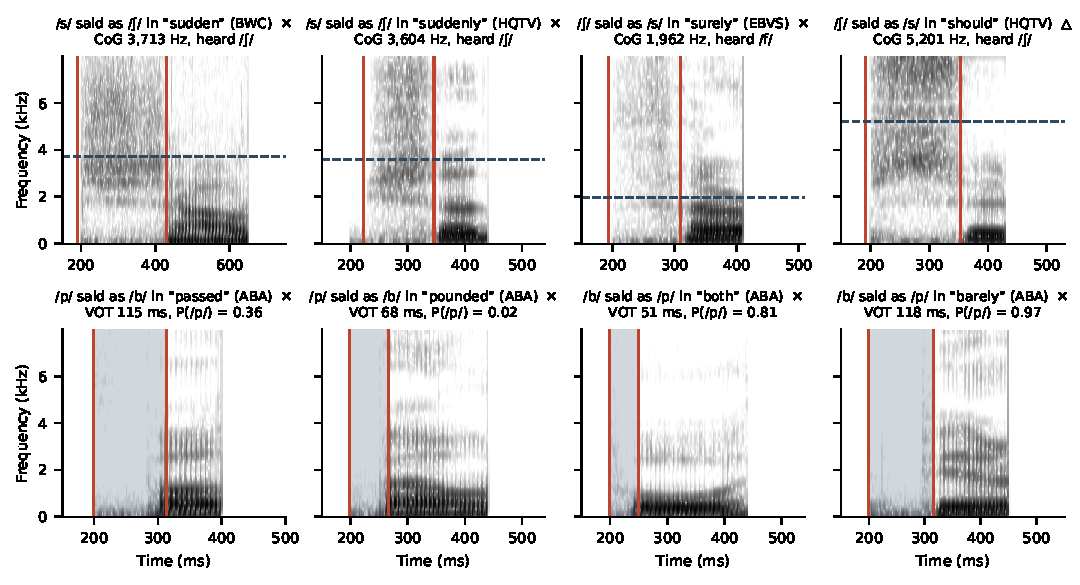
\includegraphics[width=\textwidth]{figs/fig_l2_errors.pdf}
\caption{Annotated learner substitutions in L2-ARCTIC and the verdict of the final pipeline. Top: \ipa{s} said as \ipa{\textesh} and the reverse (the last panel is a miss: the tool hears \ipa{\textesh} and gives \textit{almost}); bottom: \ipa{p} said as \ipa{b} and the reverse. In the first bottom panel the VOT is long (115~ms) although the annotators heard \ipa{b}, which is why a VOT rule alone fails.}
\label{fig:errors}
\end{figure*}

\begin{figure*}[!t]
\centering
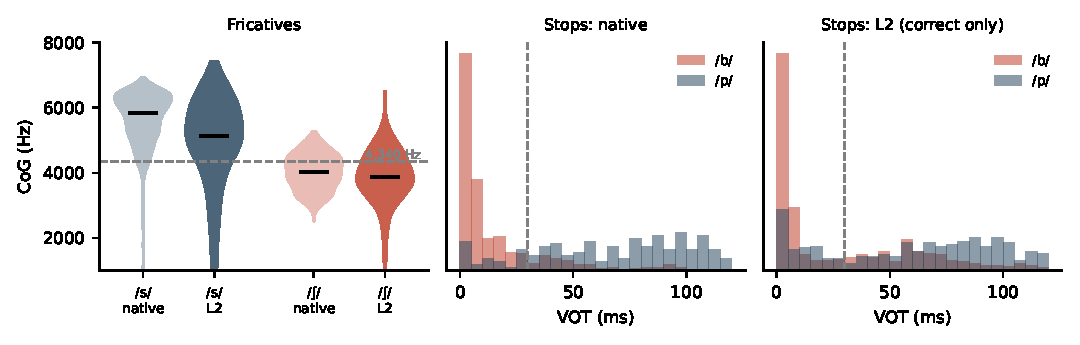
\includegraphics[width=0.92\textwidth]{figs/fig_shift.pdf}
\caption{Why native-voice rules fail for learners. Left: CoG of word-initial \ipa{s} and \ipa{\textesh} in native ARCTIC voices and in correctly produced L2 speech; the L2 \ipa{s} extends below the fixed 4{,}340~Hz threshold. Right: VOT of \ipa{p} and \ipa{b} in native and correctly produced L2 speech; the 30~ms threshold separates the learners' categories less well.}
\label{fig:shift}
\end{figure*}

\subsection{Population Shift: Native Thresholds on Learner Speech}
Table~\ref{tab:l2} and Fig.~\ref{fig:shift} show that the threshold rules, although accurate on D1, rejected 45\% of the correctly produced \ipa{s} and 43\% of the correctly produced \ipa{\textesh} of L2 speakers. The recogniser-assisted design reduced these false rejections to 8\% and 3\%, respectively, and the annotated errors were retained at 100\% and 88\%. For the four Vietnamese speakers, the corresponding false-rejection rates were 7\% and 3\%, with 16/16 and 28/30 errors retained. It is concluded that, for these two sounds, native-voice thresholds are not sufficient, and that an additional decision on the identity of the sound is required.

\begin{table}[!htb]
\caption{Fricative errors in L2-ARCTIC: false rejection of correct productions (FR) and detection of annotated errors (Det.). Wilson 95\% intervals in brackets.}
\label{tab:l2}
\centering
\small
\begin{tabular}{llcc}
\toprule
Sound & Scoring & FR (correct) & Det. (errors) \\
\midrule
\multirow{2}{*}{\ipa{s}} & Thresholds & 45\% [42, 49] & 83\% [61, 94] \\
 & Recogniser-assisted & 8\% [6, 10] & 100\% [82, 100] \\
 & \scriptsize{$n$ (correct / error)} & \scriptsize{861} & \scriptsize{18} \\
\midrule
\multirow{2}{*}{\ipa{\textesh}} & Thresholds & 43\% [39, 47] & 84\% [68, 93] \\
 & Recogniser-assisted & 3\% [2, 5] & 88\% [72, 95] \\
 & \scriptsize{$n$ (correct / error)} & \scriptsize{602} & \scriptsize{32} \\
\bottomrule
\end{tabular}
\end{table}

\subsection{Stops}
For \ipa{p} and \ipa{b}, a fixed VOT threshold of 30~ms gave a balanced accuracy of 0.88 on native speech, but on L2 speech it was a weak detector (Table~\ref{tab:stops}). The probe trained on native speech (balanced accuracy 0.96, leave-one-voice-out) detected 85\% of the annotated \ipa{p} errors, most of which were \ipa{p} produced as \ipa{b}, compared with 43\% for the VOT rule, and it reduced the false-rejection rate of \ipa{b} from 39\% to 10\%. However, 36\% of the correctly annotated \ipa{p} were still rejected, and part of this may reflect weakly aspirated productions that the annotators accepted. The detection of \ipa{b} errors rests on 26 cases only.

\begin{table}[!htb]
\caption{Stops in L2-ARCTIC: VOT rule versus recogniser probe.}
\label{tab:stops}
\centering
\small
\begin{tabular}{llcc}
\toprule
Sound & Scoring & FR (correct) & Det. (errors) \\
\midrule
\ipa{p} & VOT $\geq$ 30 ms & 28\% [24, 34] & 43\% [33, 54] \\
($n$ = 309 / 86) & Probe & 36\% [31, 41] & 85\% [76, 91] \\
\midrule
\ipa{b} & VOT $<$ 30 ms & 39\% [36, 42] & 46\% [29, 65] \\
($n$ = 962 / 26) & Probe & 10\% [8, 12] & 54\% [35, 71] \\
\bottomrule
\end{tabular}
\end{table}

\subsection{Context Leakage in Recogniser Evaluation}
When applied to whole words of eight native voices, the recogniser separated \ipa{f} from \ipa{\texttheta} with an accuracy of 0.99. Because the recogniser reads the entire clip, this figure may reflect the remainder of the word, and three controls were therefore applied. With the hiss alone, \ipa{f}--\ipa{\texttheta} accuracy fell to 0.67, whereas \ipa{s}--\ipa{\textesh} accuracy remained at 0.94. When the hiss of one sound was spliced into a word beginning with the other (320 splices per case), the recogniser followed the word rather than the hiss in 69--73\% of the \ipa{f}--\ipa{\texttheta} cases, but followed the hiss in 73--90\% of the \ipa{s}--\ipa{\textesh} cases. At a signal-to-noise ratio of 10~dB, \ipa{f}--\ipa{\texttheta} accuracy was 0.71. It follows that recogniser accuracy measured on words overstates its ability to discriminate the consonant itself for the \ipa{f}--\ipa{\texttheta} pair, and that this pair cannot currently be scored reliably from the hiss; it is therefore not graded.

\begin{figure}[!htb]
\centering
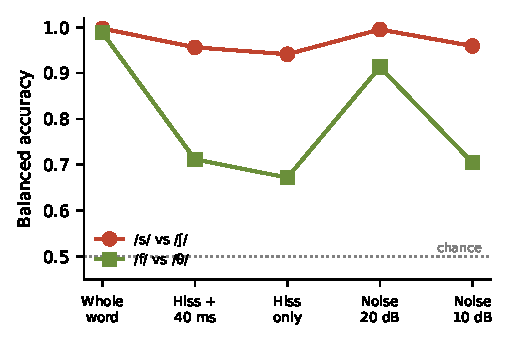
\includegraphics[width=0.85\columnwidth]{figs/fig_context.pdf}
\caption{Recogniser accuracy for \ipa{s}--\ipa{\textesh} and \ipa{f}--\ipa{\texttheta} as the context is removed or noise is added (eight native voices). The \ipa{f}--\ipa{\texttheta} contrast depends on the surrounding word.}
\label{fig:context}
\end{figure}

\subsection{Other Sounds and Personalisation}
For \ipa{m} and \ipa{n}, formant measures with Praat reached only 0.63 balanced accuracy on native speech, and the recogniser reached 0.98 on the words \textit{me} and \textit{knee}, which share the vowel and therefore do not reveal the answer through context. For \ipa{t\textesh} against \ipa{\textesh}, the recogniser probe reached 0.96 end-to-end (hand-crafted rise-time features: 0.80). Fewer than six annotated learner errors are available for \ipa{t\textesh}, \ipa{m}, \ipa{n}, and \ipa{f}, so that no error-detection rate is reported for them. For \ipa{s} against \ipa{\textesh}, per-speaker normalisation raised balanced accuracy from 0.90 to 0.97 across eight native voices, and six calibration recordings sufficed (0.95 end-to-end).

\section{Discussion and Limitations}\label{sec:disc}
The principal finding is that validation on native speech is not sufficient for an assistive pronunciation tool, because a measure that agrees with expert manual measurement can nevertheless reject a substantial share of correct learner productions. Furthermore, the context-controlled tests show that the choice of evaluation unit influences the conclusion about a recogniser. In practical terms, a design in which the identity of the sound is decided by a recogniser and the degree of correctness by interpretable acoustic measures retains the visual transparency that DHH learners and teachers require.

Several limitations must be stated. First, no DHH learner has yet used the tool, and the L2 speakers of the corpus are hearing speakers; the findings therefore cannot be generalised to DHH speech, which may differ in pitch, intelligibility, and breathiness. Second, all consonants were cut from continuous sentences, not recorded as isolated words. Third, the annotated errors are few for several sounds, and the annotation reflects perceptual judgement by listeners, which may favour a recogniser trained on phonemic transcriptions. Fourth, the thresholds and confidence values are provisional, and the displayed confidence is a model score, not a calibrated probability. Fifth, the recogniser branch requires the model to be installed, and the learner must leave a short pause before the word. In addition, the boundary detector can mislocate the hiss (for example, a \ipa{\textesh} in ``sure'' was measured at a CoG of 368~Hz), and in such a case the recogniser's decision, not the measurement, determines the verdict. Finally, learning outcomes have not been measured.

\section{Pilot Study}

The pilot has two strands with different questions. The teacher strand asks
whether the feedback is clear and useful. The learner strand asks whether the
tool's verdicts agree with a teacher's judgement of the same recordings.

\subsection{Teacher Strand}
Teachers of English or speech-language specialists who work with deaf and
hard-of-hearing (DHH) learners are invited \tbd{number, recruiting site,
years of experience}. After a short demonstration, each teacher uses the
tool with the eight target words (/s/, \ipa{\textesh}, \ipa{t\textesh}, /f/, /m/, /n/, /p/, /b/)
 and then completes a short questionnaire on the
clarity of the three-level verdict and the spectrogram and on the usefulness
of the measures and tips \tbd{items, scale, source of any adapted
instrument}. Open comments are coded thematically \tbd{coding procedure}.

\subsection{Learner Strand}
Learners record the eight target words as single words
\tbd{population: hearing EFL learners first; DHH learners, including children
with cochlear implants, conditional on ethical approval and consent;
number, age range}. At least two teachers, blind to the tool's verdicts,
rate each target consonant as correct, almost, or not yet
\tbd{scale, rater training, number of raters}. Agreement between the tool and
the teachers is compared with agreement between the teachers
\tbd{statistic, e.g., weighted kappa}. Recording conditions follow
Section~\ref{sec:data} \tbd{fix label}.

\subsection{Ethics}
\tbd{ethical approval number, informed consent for adults, parental consent
and child assent where learners are minors, data storage and anonymisation}.

\subsection{Results}
\tbd{participant numbers, questionnaire results, tool--teacher and
teacher--teacher agreement, summary of comments}.

\section{Conclusion}
A visual pronunciation feedback tool for eight English consonants was described and evaluated on annotated learner speech. Thresholds validated on native voices over-rejected correct productions, whereas a recogniser-assisted design reduced false rejection for \ipa{s} and \ipa{\textesh} to 8\% and 3\% without losing the annotated confusions, and a probe improved the detection of \ipa{p}--\ipa{b} errors. The \ipa{f}--\ipa{\texttheta} contrast could not be established from the consonant alone. Future work comprises recording isolated words from native, L2, and DHH speakers, repeating the evaluation on that material, and measuring the effect of the feedback on learning.

\section*{Acknowledgment}
\tbd{Funding and acknowledgements (FTIP project, National Formosa University).}

\begin{thebibliography}{00}
% The first five entries below were written from memory (Jongman, Baevski, Xu, Zhao, Kominek): verify before submission. The others were taken from the PDFs in literatures/.
\bibitem{jongman2000} A. Jongman, R. Wayland, and S. Wong, ``Acoustic characteristics of English fricatives,'' \textit{J. Acoust. Soc. Am.}, vol. 108, no. 3, pp. 1252--1263, 2000.
\bibitem{baevski2020} A. Baevski, H. Zhou, A. Mohamed, and M. Auli, ``wav2vec 2.0: A framework for self-supervised learning of speech representations,'' in \textit{Proc. NeurIPS}, 2020.
\bibitem{xu2022} Q. Xu, A. Baevski, and M. Auli, ``Simple and effective zero-shot cross-lingual phoneme recognition,'' in \textit{Proc. Interspeech}, 2022.
\bibitem{zhao2018} G. Zhao \textit{et al.}, ``L2-ARCTIC: A non-native English speech corpus,'' in \textit{Proc. Interspeech}, 2018, pp. 2783--2787.
\bibitem{kominek2004} J. Kominek and A. W. Black, ``The CMU Arctic speech databases,'' in \textit{Proc. 5th ISCA Speech Synthesis Workshop}, 2004, pp. 223--224.
\bibitem{hitchcock2023} E. R. Hitchcock, J. L. Preston, L. C. Ochs, M. T. Swartz, M. C. Leece, and T. McAllister, ``Tutorial: Using visual--acoustic biofeedback for speech sound training,'' \textit{Am. J. Speech-Lang. Pathol.}, vol. 32, pp. 18--36, 2023.
\bibitem{truong2005} K. Truong, A. Neri, F. de Wet, C. Cucchiarini, and H. Strik, ``Automatic detection of frequent pronunciation errors made by L2-learners,'' in \textit{Proc. Interspeech}, 2005.
\bibitem{moradi2017} S. Moradi, B. Lidestam, H. Danielsson, E. H. N. Ng, and J. R{\"o}nnberg, ``Visual cues contribute differentially to audiovisual perception of consonants and vowels in improving recognition and reducing cognitive demands in listeners with hearing impairment using hearing aids,'' \textit{J. Speech Lang. Hear. Res.}, vol. 60, pp. 2687--2703, 2017.
\bibitem{desai2008} S. Desai, G. Stickney, and F.-G. Zeng, ``Auditory-visual speech perception in normal-hearing and cochlear-implant listeners,'' \textit{J. Acoust. Soc. Am.}, vol. 123, no. 1, pp. 428--440, 2008.
\bibitem{winn2013} M. B. Winn, A. E. Rhone, M. Chatterjee, and W. J. Idsardi, ``The use of auditory and visual context in speech perception by listeners with normal hearing and listeners with cochlear implants,'' \textit{Front. Psychol.}, vol. 4, art. 824, 2013.
\bibitem{pimperton2017} H. Pimperton, A. Ralph-Lewis, and M. MacSweeney, ``Speechreading in deaf adults with cochlear implants: Evidence for perceptual compensation,'' \textit{Front. Psychol.}, vol. 8, art. 106, 2017.
\bibitem{ertmer2011} D. J. Ertmer and L. Goffman, ``Speech production accuracy and variability in young cochlear implant recipients: Comparisons with typically developing age-peers,'' \textit{J. Speech Lang. Hear. Res.}, vol. 54, no. 1, pp. 177--189, 2011.
\bibitem{kim2025} S.-E. Kim, B. R. Chernyak, J. Keshet, M. Goldrick, and A. R. Bradlow, ``Predicting relative intelligibility from inter-talker distances in a perceptual similarity space for speech,'' \textit{Psychon. Bull. Rev.}, vol. 32, pp. 1664--1675, 2025.
\bibitem{kuperman2012} V. Kuperman, H. Stadthagen-Gonzalez, and M. Brysbaert, ``Age-of-acquisition ratings for 30,000 English words,'' \textit{Behav. Res. Methods}, vol. 44, pp. 978--990, 2012.
\bibitem{stelmachowicz2004} P. G. Stelmachowicz et al., ``The importance of high-frequency audibility in the speech and language development of children with hearing loss'', \textit{Arch. Otolaryngol. Head Neck Surg.}, vol. 130, no. 5, pp. 556--562, 2004, doi: 10.1001/archotol.130.5.556.
\bibitem{yang2017} J. Yang, J. Vadlamudi, Z. Yin, C.-Y. Lee, and L. Xu, ``Production of word-initial fricatives of Mandarin Chinese in prelingually deafened children with cochlear implants'', \textit{Int. J. Speech-Lang. Pathol.}, vol. 19, pp. 153--164, 2017, doi: 10.3109/17549507.2016.1143972.
\bibitem{ertmer2004} D. J. Ertmer, ``How well can children recognize speech features in spectrograms? Comparisons by age and hearing status'', \textit{J. Speech Lang. Hear. Res.}, vol. 47, no. 3, pp. 484--495, 2004, doi: 10.1044/1092-4388(2004/038).
\bibitem{ertmermaki2000} D. J. Ertmer and J. E. Maki, ``A comparison of speech training methods with deaf adolescents: Spectrographic versus noninstrumental instruction'', \textit{J. Speech Lang. Hear. Res.}, vol. 43, no. 6, pp. 1509--1523, 2000.
\bibitem{carroll2015}
P. Carroll, J. Trouvain, and F. Zimmerer,
``A visual feedback tool for German vowel production,''
in \emph{Proc. 26th Conf. Elektronische Sprachsignalverarbeitung
(ESSV)}, Eichst{\"a}tt, Germany, 2015, pp. 150--157.
\end{thebibliography}

\end{document}
